\documentclass[acmsmall,screen,review]{acmart}
\usepackage{amsmath}
\usepackage{booktabs}
\usepackage{tabularx}
\usepackage{array}
\usepackage{tikz}
\usepackage{microtype}
\usetikzlibrary{arrows.meta,positioning,fit,calc}
\acmJournal{CSUR}
\renewcommand{\arraystretch}{1.12}
\newcolumntype{Y}{>{\raggedright\arraybackslash}X}
\newcolumntype{L}[1]{>{\raggedright\arraybackslash}p{#1}}
\newcommand{\claimlevel}[1]{\textsf{L#1}}
\newcommand{\evidence}[1]{\textsf{E#1}}
\title{From Resemblance to Authority: Claim-Bounded Evidence for Android Software Lineage in AI-Mediated Supply Chains}
\author{Haoyi Zhang}
\affiliation{\institution{Xi'an Jiaotong-Liverpool University}\city{Suzhou}\country{China}}
\email{hyeliozhang@gmail.com}
\author{Huaijin Ran}
\affiliation{\institution{Nanyang Technological University}\city{Singapore}\country{Singapore}}
\email{huaijin003@e.ntu.edu.sg}
\renewcommand{\shortauthors}{Zhang and Ran}
\IfFileExists{generated/corpus_counts.tex}{\newcommand{\CorpusWorks}{97}
\newcommand{\VenueRecordedWorks}{93}
\newcommand{\PrimaryWorks}{76}
\newcommand{\PrimaryVenueWorks}{74}
\newcommand{\SecondaryWorks}{21}
\newcommand{\ReviewMatrixWorks}{21}
\newcommand{\SourceRechecks}{26}
\newcommand{\SourceRecheckPercent}{26.8}
\newcommand{\AndroidWorks}{34}
\newcommand{\TPLWorks}{17}
\newcommand{\SupplyWorks}{17}
\newcommand{\AIWorks}{8}
\newcommand{\UniqueCitedWorks}{97}
\newcommand{\FullSelectedWorks}{61}
\newcommand{\AbstractSelectedWorks}{36}
}{%
  \newcommand{\CorpusWorks}{97}\newcommand{\UniqueCitedWorks}{97}%
  \newcommand{\VenueRecordedWorks}{93}\newcommand{\PrimaryWorks}{76}%
  \newcommand{\PrimaryVenueWorks}{74}\newcommand{\SecondaryWorks}{21}\newcommand{\ReviewMatrixWorks}{21}%
  \newcommand{\SourceRechecks}{26}\newcommand{\SourceRecheckPercent}{26.8}\newcommand{\FullSelectedWorks}{61}%
  \newcommand{\AbstractSelectedWorks}{36}\newcommand{\AndroidWorks}{34}%
  \newcommand{\TPLWorks}{17}\newcommand{\SupplyWorks}{17}%
  \newcommand{\AIWorks}{8}}
\begin{document}
\begin{abstract}
Android lineage questions are often phrased as one detection problem even though byte identity, component presence, resemblance, derivation, build provenance, release authorization, and behavioral assurance are different propositions. Existing surveys separately cover Android repackaging, third-party libraries, software-supply-chain security, and software bills of materials; this review therefore does not claim an uncovered detector literature. Instead, it asks which observation licenses which claim, under what transformation and trust assumptions, and which bindings are required when evidence is composed across layers. We code \CorpusWorks{} scholarly works, including \PrimaryWorks{} primary, empirical, or system studies, and adversarially compare \ReviewMatrixWorks{} review or method records across seven coverage dimensions. Every retained work has a claim-level extraction with an explicit counter-history and inference limit; \SourceRechecks{} load-bearing assignments receive a fresh source-grounded recheck within the same authoring process. The synthesis introduces a seven-level ladder spanning identity, composition, resemblance, derivation, process provenance, authorization, and behavioral assurance. It shows that most repackaging and component mechanisms establish resemblance or composition; derivation direction normally requires temporal, ownership, source, or authenticated process evidence. Signing, transparency, and provenance can bind principals, steps, and artifacts, but do not establish semantic equivalence or benign behavior. AI-mediated development adds sibling generations, synthesized dependencies, hidden retrieval and tool context, and model drift, making source-to-APK binding more important rather than making artifact analysis obsolete. We derive a cross-layer assurance pattern that binds transformation-aware comparison, component/version evidence, authenticated step records, release policy, and behavior-specific analysis to the same digest or documented predecessor relation. The contribution is a bounded structured evidence synthesis and evaluation blueprint, not a universal detector ranking, pooled meta-analysis, or proof of worldwide novelty.
\end{abstract}
\keywords{Android, software lineage, application repackaging, software supply chain, provenance, third-party libraries, code generation, evidence validity}
\maketitle

\section{Introduction}

Two Android packages may look alike for many legitimate and illegitimate reasons. They may be separate builds of one code base, applications that embed the same advertising library, products generated from one template, regional variants signed by different subsidiaries, siblings produced from the same prompt, or an original and an unauthorized derivative. A detector can be accurate about a shared feature while still being unable to distinguish among those histories. The central problem is therefore not merely whether two artifacts are similar. It is whether the observation is strong enough for the relationship asserted by an analyst, marketplace, developer, or incident responder.

This distinction is established indirectly across several mature literatures. Repackaging research studies code reuse, graph similarity, resource resemblance, visual clones, watermarks, and malicious grafting~\cite{droidmoss,attackclones,adrob,appink,droidmarking,piggybacking}. Third-party-library (TPL) research studies how to separate application code from reused components and identify families and versions despite shrinking, partial inclusion, and obfuscation~\cite{commonlibraries,libd,libradar,libscout,libid,atvhunter}. Software-supply-chain research instead asks who performed a step, which materials were consumed, which artifact was produced, how repository metadata was authorized, and whether different observers receive consistent histories~\cite{tuf,intoto,chainiac,sigstore,diplomat}. These bodies of work are complementary, but their guarantees do not compose automatically.

AI-mediated development makes the boundary more visible. A text-to-application system can generate compilable Android source from a natural-language description, while an agentic system can create and revise an application through multiple tool calls~\cite{text2app,appforge}. Code assistants may also introduce insecure code, propose nonexistent packages, reproduce sensitive material, or alter code through iterations whose causal history is not represented by the final APK alone~\cite{pearce,perry,sandoval,spracklen,codexleaks}. An application can therefore be novel at the byte level, similar at the behavioral or user-interface level, composed partly of inherited code, and produced through an authorized but weakly recorded process. No single binary relation captures all of those facts.

The practical consequence is a recurring category error. A high similarity score is reported as proof of copying; a component match is treated as proof of application ancestry; a valid signature is treated as proof of rightful authorization; an SBOM entry is treated as proof that the listed code is present and reachable; or a reproducible build is treated as proof that the inputs were approved. Each inference may become defensible with additional evidence, but the missing premise is often implicit. Once hidden, it is difficult to benchmark, transfer to a new workflow, or challenge during an appeal.

This survey does not claim that Android repackaging or supply-chain security lacks prior synthesis. Li, Bissyand\'e, and Klein reviewed 57 repackaging approaches and introduced RePack to expose reproducibility and comparison weaknesses~\cite{repack}. Wu et al. subsequently published a comprehensive survey of Android repackaging detection, including code- and resource-based techniques, datasets, metrics, and future directions~\cite{wurepack2026}. Zhan et al. organized 74 Android TPL studies around tasks including module separation, family identification, and version attribution, while Zeng et al. broadened the view to TPL security in application software~\cite{tpl,zengtpsurvey2024}. Recent syntheses cover software-supply-chain attacks and defenses, secure-design properties, research directions, and cyber-supply-chain risk~\cite{astra,properties,ladisa,reichert2024,williams2025,gokkaya2026,cyberrisk2026}; empirical SBOM studies additionally expose design and adoption problems in practice~\cite{bi2024sbom,bomsaway2024}. A defensible contribution must therefore be narrower than ``an updated repackaging survey'' and different from a general supply-chain taxonomy.

The question retained here is claim-centered: \emph{which observable evidence supports which Android lineage or assurance proposition, under what transformation and trust assumptions, and what bindings are required when evidence is composed across artifacts, components, build steps, release policy, behavior, and AI-mediated changes?} A bounded adversary analysis of \ReviewMatrixWorks{} review and method records found no single coded source that directly covered seven dimensions with one observation-to-claim discipline and an explicit cross-layer binding rule. This is a positioning result over the retained set, not proof that no uncoded publication contains part of the argument.

The survey answers four research questions:

\begin{description}
\item[RQ1: Claim structure.] What distinct lineage and assurance claims recur in Android analysis, and which evidence objects can support each claim?
\item[RQ2: Transformation robustness.] How do rewriting, obfuscation, resource changes, library reuse, compilation, and generation alter the validity of artifact-level evidence?
\item[RQ3: Cross-layer composition.] How can artifact analysis, component evidence, authenticated process records, release authorization, and behavior analysis be combined without overstating any layer?
\item[RQ4: AI-mediated development.] Which assumptions become fragile when source and mobile artifacts are generated or revised through nondeterministic, tool-using systems?
\end{description}

The review contributes a seven-level claim ladder; a mechanism map linking objects, transformations, oracles, ceilings, and counter-histories; a digest-bound cross-layer assurance pattern; and an analysis of AI-mediated sibling generation, synthesized dependencies, hidden context, tool state, and model drift. The ladder adds propositions rather than ranking every higher level as universally better.

The evidence base contains \CorpusWorks{} works, including \PrimaryWorks{} primary/system studies and \SecondaryWorks{} review/method sources. Every record has a claim-level extraction and inference limit; \SourceRechecks{} load-bearing assignments received same-process source rechecks. The counts are not a complete search denominator or independent dual coding.

The synthesis is that lineage evidence is \emph{non-substitutable}: artifact and component evidence recover relationships when process records are absent; authenticated records establish direction and accountability; release controls bind distribution authority; and behavior analysis addresses security properties. Composition strengthens assurance only when artifacts, principals, times, policies, and transformations are explicitly bound.

Section~\ref{sec:method} gives the review design. Sections~\ref{sec:model}--\ref{sec:ai} develop the claim model and domain syntheses; Sections~\ref{sec:synthesis} and~\ref{sec:agenda} derive the cross-layer blueprint and agenda.

\section{Review Design and Corpus}
\label{sec:method}

\subsection{Review type, objective, and unit of analysis}

This work is a bounded, claim-centered structured evidence synthesis, not a PRISMA-complete review or prevalence meta-analysis. Its analytic unit is a scholarly work contributing an Android artifact-comparison, component/version, provenance or reproducibility mechanism; an empirical supply-chain or AI-development study; or a structuring review or method source.

The coded unit relates object, observation, transformation model, oracle or policy, claim ceiling, and counter-history. Tool-level coding would hide stages such as module separation, signature construction, and version comparison; feature-level coding alone would also hide that clone pairs, family labels, repositories, signed policies, and rebuilds establish different propositions.

\subsection{Search, snowballing, and corpus construction}

Seeds included the Android repackaging benchmark review~\cite{repack}, the Android TPL review~\cite{tpl}, broader Android surveys~\cite{sufatrio,xuandroid,tamandroid}, and static-analysis/testing reviews~\cite{staticandroid,androidtesting}. Backward and targeted forward snowballing followed supply-chain attacks, secure design, authenticated updates, provenance, transparency, reproducible builds, CI, package ecosystems, SBOMs, and AI-mediated development, guided by established review methods~\cite{wohlin,kitchenham,brereton}.

A 2024--2026 adversarial update added direct or adjacent syntheses~\cite{wurepack2026,zengtpsurvey2024,reichert2024,williams2025,gokkaya2026,cyberrisk2026} and empirical SBOM studies~\cite{bi2024sbom,bomsaway2024}. A candidate SBOM review was excluded after its official record reported withdrawal and no paper was available for coding. The artifact preserves 105 screening decisions plus source-location and retrospective discovery rows for every retained work; these support record audit, not a database-hit denominator.

The map contains \CorpusWorks{} works: \PrimaryWorks{} primary/system and \SecondaryWorks{} review/method records. \PrimaryVenueWorks{} primary/system and \VenueRecordedWorks{} total records are venue-published; the remainder are three preprints and one method report. Coding depth is \FullSelectedWorks{} full-or-selected-source and \AbstractSelectedWorks{} abstract-or-selected-passage records, with ceilings limited accordingly.

\begin{table}[t]
\caption{Corpus strata and their role. Counts describe the retained evidence map, not field prevalence.}
\label{tab:corpus}
\small
\begin{tabularx}{\textwidth}{L{2.65cm}rY Y}
\toprule
Stratum & Works & Main evidence objects & Principal use \\
\midrule
Android artifact analysis & \AndroidWorks & DEX code, graphs, resources, UI, behavior, signatures, clone pairs & Bound artifact-level identity, resemblance, and directional claims \\
Third-party libraries & \TPLWorks & Module boundaries, signatures, versions, update histories & Separate composition, version, reachability, and application ancestry \\
Supply-chain integrity & \SupplyWorks & Metadata, attestations, logs, roles, builds, CI workflows & Establish principals, steps, authorization, transparency, and reproducibility \\
AI-mediated development & \AIWorks & Prompts, generated source, dependencies, interactions, accepted output & Identify generated transformations, missing context, and causal-record limits \\
Reviews and method & \SecondaryWorks & Taxonomies, protocols, benchmark critiques, design properties & Adversarially position scope and normalize evaluation obligations \\
\bottomrule
\end{tabularx}
\end{table}

The heterogeneous corpus is not pooled into a detector ranking: candidate generation, transformations, labels, periods, and counting units differ, and benchmark construction can dominate apparent results~\cite{repack,repackeval,blackburn}. The synthesis therefore compares mechanisms and inference validity.

\subsection{Corpus records}

The evidence package separates the representation consumed for coding from the canonical bibliographic record. Each retained work has a corpus row, BibTeX entry, source-location boundary, retrospective discovery row, and publication-status record. DOI-bearing entries use the DOI as canonical identifier; other records use an official venue, archive, or report locator. Automated checks require title and year agreement, unique identifiers, and consistency between venue/preprint status and entry type. A withdrawn SBOM candidate is preserved only in an exclusion ledger and historical regression fixture. These checks establish record-level consistency, not a comprehensive retraction-registry search or independent confirmation of every interpretation.

\subsection{Prior-review adversary matrix}

Each of \ReviewMatrixWorks{} review/method records was coded for Android repackaging, component/version evidence, provenance, authorization, behavior, AI mediation, and an explicit claim ceiling with cross-layer binding. Table~\ref{tab:review-matrix} uses 1 for direct treatment, P for partial, 0 for out of scope, and ? for unresolved; the artifact retains every row and source basis.

\begin{table}[t]
\caption{Selected prior-review adversary matrix. A=Android repackaging, C=component/version, P=process provenance, U=authorization, B=behavior, G=AI-mediated generation, X=claim-ceiling and binding rule.}
\label{tab:review-matrix}
\centering
\scriptsize
\begin{tabular}{lccccccc}
\toprule
Prior synthesis & A & C & P & U & B & G & X \\
\midrule
\input generated/review_matrix_rows.tex
\bottomrule
\end{tabular}
\end{table}

No retained row directly covers all seven dimensions under one inference rule. This rejects a broad ``no prior survey'' claim while supporting the narrower organizing question. Partial cells prevent absence-by-title reasoning, and uncoded work remains possible; the matrix is positioning evidence, not worldwide novelty proof.

\subsection{Inclusion, exclusion, and source-depth rules}

Works were included when their technical object could support an Android lineage or release claim. Clone/malware systems supplied reusable artifact observations; supply-chain systems supplied source, build, repository, or release evidence; and AI papers generated mobile software or measured security-relevant generation workflows. General model, GUI-agent, or prompt-injection work without a software-artifact lineage object was excluded.

Publication status and evidential role were separate. Preprints may expose emerging workflows, and method reports may guide procedure, without counting as peer-reviewed primary evidence. Every record has a scholarly/official locator and version-status row; withdrawn or retracted candidates are quarantined. This is not a comprehensive retraction-registry search, and lighter-depth records are limited to what their accessible materials support.

\subsection{Claim-level extraction and recheck}

Each retained work has seven recorded fields: the evidence object, observation, transformation model, oracle or policy, claim ceiling, counter-history, and inference limit. Source-specific statements are distinguished from broad stratum categories: a category such as ``renaming or library reuse'' does not establish that the cited study tested every listed transformation. Counter-histories and inference limits are our analytical classifications, not empirical findings attributed to the source. Similarity alone establishes resemblance; direction requires chronology, source, ownership, or provenance. Authenticated builds do not prove safety, and family, version, and reachability remain distinct.

Three source-specific examples illustrate the distinction. FlowDroid concerns context-, flow-, field-, and object-sensitive taint analysis of Android callbacks and lifecycle behavior~\cite{flowdroid}; it is not a renaming experiment merely because it shares the Android-artifact stratum. LibScout uses dependency analysis and application/library profiles to identify third-party libraries despite transformations addressed by its matching design~\cite{libscout}. ATVHunter combines library identification with version-sensitive analysis, so library presence alone does not establish its version-level conclusion~\cite{atvhunter}. Their extraction rows now name the actual source sections and evaluated conditions. The other broad-category fields organize candidate mechanisms but do not enumerate every transformation tested by each source; this synthesis does not infer a per-operator robustness result from those fields.

\SourceRechecks{} extractions (\SourceRecheckPercent\%) received source-grounded rechecks, prioritizing direct adversaries and high-load assignments. Rechecks record the old and revised ceiling, source, result, and boundary; they are same-process checks, not independent coding.

\subsection{Evidence-strength notation}

The claim ladder states \emph{which proposition} is supported; an orthogonal grade states \emph{how it was evaluated}.

\begin{table}[t]
\caption{Evidence-strength notation. A higher grade is not automatically available for every question.}
\label{tab:evidence-grades}
\small
\begin{tabularx}{\textwidth}{L{.85cm}L{2.85cm}Y Y}
\toprule
Grade & Evaluation basis & Typical strength & Typical limitation \\
\midrule
\evidence{0} & Illustrative example & Makes a mechanism concrete & No discriminating evaluation \\
\evidence{1} & Curated positive cases & Demonstrates feasibility & Does not estimate false positives or open-world behavior \\
\evidence{2} & Positive and negative labeled corpus & Supports discrimination under a stated oracle & Labels may encode the method's assumptions \\
\evidence{3} & Transformation-aware or adversarial corpus & Tests robustness to explicit changes & Covers a finite transformation family \\
\evidence{4} & Temporal, cross-market, or independently constructed validation & Reduces leakage and construction bias & Transfer beyond sampled ecosystems remains uncertain \\
\evidence{5} & Authenticated process evidence or independent reproduction & Supports a stated provenance or equality proposition & Does not imply semantic safety or policy authorization \\
\bottomrule
\end{tabularx}
\end{table}

The two axes must remain separate. A valid signature may strongly bind a key and artifact while saying nothing about functional equivalence. A transformation-aware benchmark can strongly evaluate resemblance robustness without identifying the authorized publisher.

\subsection{Synthesis and contradiction procedure}

Synthesis first grouped observation families, then assigned each a ceiling and counter-history, and finally mapped the bindings needed across the Android lifecycle. Contradictions denote incompatible objects, denominators, times, policies, or oracles rather than numerical disagreement alone. This is not vote counting: repeated observations cannot convert resemblance into direction or provenance into benign behavior. Seven synthesis propositions retain named support, counter-histories, and boundaries in the claim ledger.

\subsection{Deterministic traceability and negative controls}

The standalone artifact checks one-to-one bindings among corpus, bibliography, extraction, source-location, provenance, status, screening, recheck, calibration, and material-claim ledgers. It rejects duplicate keys or canonical identifiers, title/year drift, missing source boundaries, publication-type conflicts, stale leads, generic extraction templates, or leakage of an excluded publication into active synthesis data. Mutation tests deliberately introduce representative faults to confirm that the checks fail rather than merely report success on the supplied files.

A retained historical gap pilot also exercises unknown handling. Its exhaustive $3\times3$ ternary-matrix oracle compares the implemented direct/mosaic classification with an independently expressed completion rule over every small case. This finite check validates bookkeeping semantics only; it does not prove literature completeness, source interpretation, or any detector guarantee. Keeping manuscript totals current requires rerunning the checks and regenerating tables and count macros on the current evidence map before building. The ordinary paper build imports existing fragments; it does not itself enforce their freshness against current inputs.

The offline reproduction passes 61 unit and mutation tests without skips
across five serial commands. Corpus checks retain all 97 coded records;
finite oracles cover 19,683 ternary matrices and 262,144 binary completions
without disagreement. These are record-consistency and bookkeeping checks,
not an additional source-reading or independent coding pass.

\subsection{Validity limits}

The map is not an exhaustive detector census: it lacks a complete search denominator, independent second coder, pooled accuracy estimate, and prevalence claim; some records remain at abstract-plus-selected-passage depth. The adversary matrix and rechecks reduce obvious errors but cannot prove worldwide absence or independent interpretation.

\section{An Evidence Model for Mobile Software Lineage}
\label{sec:model}

\subsection{Why lineage is not one relation}

The term \emph{lineage} is used for at least four different relations. A structural relation states that two artifacts share material. A historical relation states that one artifact was derived from another or that both descend from a common source. A procedural relation states that an artifact was produced by a recorded sequence of steps and principals. A normative relation states that the production or release was authorized. Security and policy questions add a fifth relation concerning behavior. These relations can coincide, but none entails all the others.

Let an evidence item be represented as
\[
  e=(o,\phi,r,m,q,a),
\]
where $o$ is the observed object, $\phi$ is the feature or record extracted from it, $r$ is the relation being inferred, $m$ is the transformation model, $q$ is the oracle or policy against which the inference is evaluated, and $a$ is the set of assumptions. The tuple is not a new detector. It is a discipline for stating what a detector or provenance mechanism actually observes.

For example, a fuzzy code signature may compare methods after identifier normalization. Here, $o$ is DEX method code, $\phi$ is a normalized signature, $m$ includes identifier renaming but may exclude control-flow restructuring, and $q$ may be a corpus of known repackaged pairs. The supported relation is resemblance under $m$. Direction is not part of that observation unless the oracle or auxiliary evidence supplies it. By contrast, an in-toto link observes authenticated step metadata and binds materials to products under a layout~\cite{intoto}. It supports a process relation under key, layout, and metadata assumptions, but does not establish that two programs are semantically equivalent.

\subsection{The seven-level claim ladder}

Figure~\ref{fig:ladder} summarizes seven claim levels. The levels are not a maturity model. They are ordered so that a reader can see which additional proposition is introduced at each step.

\begin{figure}[t]
\centering
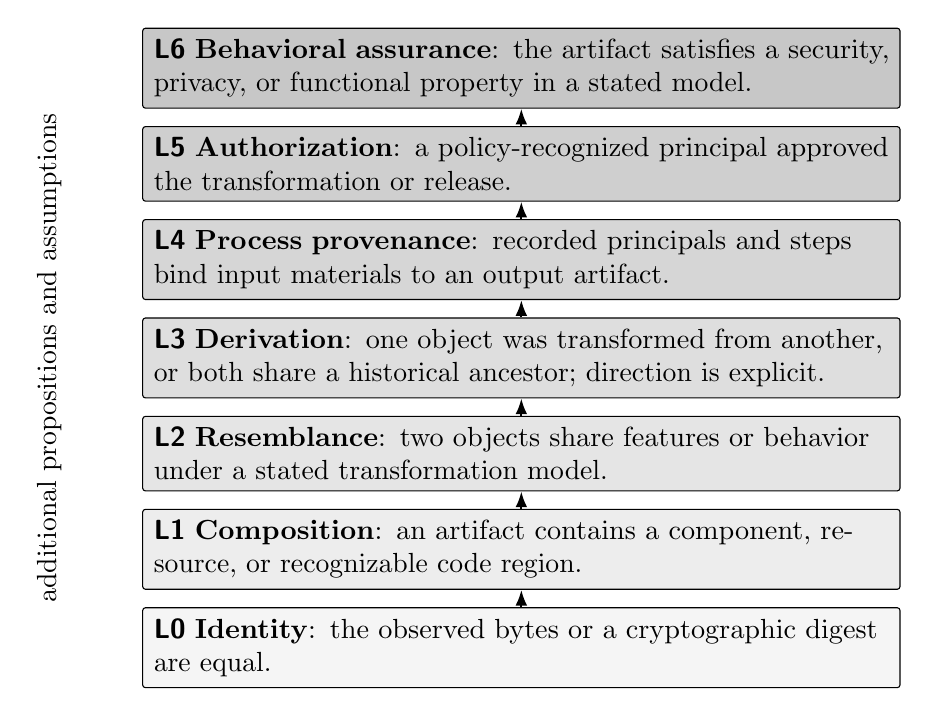
\begin{tikzpicture}[
  box/.style={draw,rounded corners=1pt,align=left,text width=.77\textwidth,minimum height=8mm,inner sep=4pt},
  arr/.style={-{Latex[length=2mm]},thick},
  node distance=2.2mm
]
\node[box,fill=black!4] (l0) {\textbf{\claimlevel{0} Identity}: the observed bytes or a cryptographic digest are equal.};
\node[box,fill=black!7,above=of l0] (l1) {\textbf{\claimlevel{1} Composition}: an artifact contains a component, resource, or recognizable code region.};
\node[box,fill=black!10,above=of l1] (l2) {\textbf{\claimlevel{2} Resemblance}: two objects share features or behavior under a stated transformation model.};
\node[box,fill=black!13,above=of l2] (l3) {\textbf{\claimlevel{3} Derivation}: one object was transformed from another, or both share a historical ancestor; direction is explicit.};
\node[box,fill=black!16,above=of l3] (l4) {\textbf{\claimlevel{4} Process provenance}: recorded principals and steps bind input materials to an output artifact.};
\node[box,fill=black!19,above=of l4] (l5) {\textbf{\claimlevel{5} Authorization}: a policy-recognized principal approved the transformation or release.};
\node[box,fill=black!22,above=of l5] (l6) {\textbf{\claimlevel{6} Behavioral assurance}: the artifact satisfies a security, privacy, or functional property in a stated model.};
\draw[arr] (l0)--(l1);\draw[arr] (l1)--(l2);\draw[arr] (l2)--(l3);\draw[arr] (l3)--(l4);\draw[arr] (l4)--(l5);\draw[arr] (l5)--(l6);
\node[align=center,rotate=90,anchor=south] at ([xshift=-9mm]l3.west) {additional propositions and assumptions};
\end{tikzpicture}
\caption{Claim ladder for Android lineage and assurance. Moving upward adds a different proposition; it is not justified merely by increasing a similarity score. Behavioral assurance is shown last because it often depends on history and policy, but it remains logically distinct from them.}
\Description{Seven stacked boxes progress from byte identity through composition, resemblance, derivation, process provenance, authorization, and behavioral assurance. An upward arrow indicates that each level adds propositions and assumptions.}
\label{fig:ladder}
\end{figure}

\paragraph{\claimlevel{0}: Identity.}
Cryptographic hashes, package digests, and reproducible-build comparisons can establish equality of the observed bytes with negligible collision probability under the selected hash assumptions. Identity is useful for artifact distribution and cache verification. It does not reveal why the bytes are equal, who authorized them, or whether they are safe. Two parties can distribute the same malicious binary.

\paragraph{\claimlevel{1}: Composition.}
Component detectors, software bills of materials, package manifests, and static analyses address whether an artifact contains a component or a recognizable region. Android library research shows that composition is itself difficult because package structure can be flattened, names can be changed, dead code can be removed, and a library can be partially embedded~\cite{tpl,libscout,libid,orlis}. Composition also has granularity: identifying a library family is weaker than identifying an exact version, and identifying bytes is weaker than showing that vulnerable code is reachable.

\paragraph{\claimlevel{2}: Resemblance.}
Most clone and repackaging detectors occupy this level. They establish that code, graphs, resources, UI, or behavior are similar under a threshold and transformation model. DroidMOSS, Juxtapp, AnDarwin, WuKong, SimiDroid, and related systems illustrate different feature choices~\cite{droidmoss,juxtapp,andarwin,wukong,simidroid}. Resemblance can be highly probative, particularly when independent feature families agree, but it does not by itself provide direction.

\paragraph{\claimlevel{3}: Derivation.}
A derivation claim states that $B$ descends from $A$, that $A$ descends from $B$, or that both descend from a specified ancestor. Direction can come from trusted timestamps, source history, market chronology, embedded marks, authenticated build records, or a curated benchmark whose construction establishes the relationship. Without such evidence, a shared library, template, or predecessor remains an alternative explanation. Repackaging papers often use known pairs or market metadata to operationalize derivation, but the feature detector and the pair-construction oracle should be reported separately~\cite{repack,repackeval}.

\paragraph{\claimlevel{4}: Process provenance.}
Process provenance binds materials, commands, environments, and principals to products. in-toto links and layouts are a direct example~\cite{intoto}; CI workflow studies show why the integrity of the recording and execution environment also matters~\cite{githubci}. Provenance can make direction explicit because it records a step from inputs to output. It remains conditional on key control, policy, collection completeness, and the absence of unrecorded paths.

\paragraph{\claimlevel{5}: Authorization.}
Authorization adds a policy judgment: the principal was allowed to perform or approve the step or release. TUF's delegated roles and Diplomat's repository delegations exemplify policy-scoped authority~\cite{tuf,diplomat}. An Android APK signature establishes possession of a signing key for that package artifact; whether the key holder is the rightful publisher is an external identity and policy question. Authorization is therefore not reducible to the presence of any valid signature.

\paragraph{\claimlevel{6}: Behavioral assurance.}
Security, privacy, and functionality concern what the artifact does. Static taint analysis, malware classification, policy analysis, dynamic testing, and formal verification can support such claims under their models~\cite{flowdroid,drebin,mamadroid}. A provenance record may help select the artifact and inputs to analyze, but it cannot replace the behavior analysis. Conversely, a behavior detector may find malicious functionality without reconstructing the artifact's full history.

\subsection{A worked claim-adjudication example}

Consider two Android packages, $A$ and $B$, collected from different channels. Their digests differ; both contain the same advertising-library family; normalized first-party call graphs, layouts, and images correspond after localization. Package $A$ also has an attested build from a named source revision and a store release under a delegated publisher role. Package $B$ uses another key and lacks an authenticated production record. Dynamic analysis reports that $B$ contacts an additional endpoint. This synthetic example illustrates adjudication rather than reporting a measurement.

The observations license separate statements. Different digests reject \claimlevel{0} identity. The shared library supports family-level \claimlevel{1} composition while leaving version, modification, and reachability unresolved. Agreement across first-party code and resources supports \claimlevel{2} resemblance under the detector's transformation model, but does not select a direction: a common template, common predecessor, authorized fork, and copying either way remain compatible histories. The authenticated record supports \claimlevel{4} only for the materials, steps, principals, and product digest it names; delegation can add scoped \claimlevel{5} authorization for $A$. Neither claim transfers to $B$, and a different valid key is not by itself proof of unauthorized release. The endpoint finding is a \claimlevel{6} observation about the analyzed build and environment, not a derivation oracle.

Later evidence should revise only the subclaim it resolves. An authenticated parent and ordered transformation could establish directional \claimlevel{3} or process-level \claimlevel{4}; a shared authenticated predecessor would instead establish sibling derivation. The correct report therefore preserves competing histories, binds every result to its exact object, and keeps retrieval, historical adjudication, authorization, and behavior distinct even when a store policy combines them into one action.

\subsection{Claim ceilings of common evidence objects}

Table~\ref{tab:claim-ceilings} records typical claim ceilings. ``Typical'' matters: an implementation can combine additional evidence and move beyond the base ceiling. The purpose is to prevent that additional evidence from disappearing inside the name of the base mechanism.

\begin{table}[t]
\caption{Typical claim ceilings and missing links. The last column names the evidence normally required for a stronger inference.}
\label{tab:claim-ceilings}
\small
\begin{tabularx}{\textwidth}{L{3cm}L{1.25cm}Y Y}
\toprule
Evidence object & Ceiling & What it directly supports & Evidence needed for a stronger claim \\
\midrule
Exact digest or byte comparison & \claimlevel{0} & Identity of observed bytes & Authenticated origin, policy, or behavior analysis \\
Component signature or SBOM entry & \claimlevel{1} & Component presence or asserted composition & Exact version, reachability, and authenticated generation \\
Code, graph, resource, UI, or trace similarity & \claimlevel{2} & Resemblance under a feature and transformation model & Directional oracle, chronology, ownership, or process record \\
Known original--derivative pair & \claimlevel{3} & Derivation for the constructed pair & Generalization to open-world candidates and authorization \\
Authenticated step attestation & \claimlevel{4} & Recorded input--step--output relation and principal & Authorization policy, complete capture, and trusted execution \\
Delegated signature or release approval & \claimlevel{5} & Policy-scoped authorization of metadata or artifact & Semantic equivalence, vulnerability, privacy, and behavior evidence \\
Static, dynamic, or formal behavior evidence & \claimlevel{6} & Property within the analysis or test model & Broader environment coverage and provenance of analyzed inputs \\
\bottomrule
\end{tabularx}
\end{table}

\subsection{Counter-histories as a validity test}

A useful way to evaluate an inference is to construct a counter-history: a plausible history that produces the observation but falsifies the claimed relation. Four counter-histories recur.

\emph{Common-predecessor ambiguity} occurs when two applications inherit code from an earlier version or template. Pairwise similarity cannot establish which is the source. \emph{Component contamination} occurs when a large shared library dominates the feature space and makes otherwise unrelated apps appear close. \emph{authorized divergence} occurs when a legitimate maintainer refactors, obfuscates, localizes, or regenerates an application so heavily that its authorized successor looks dissimilar. \emph{authenticated malice} occurs when a compromised or maliciously authorized pipeline produces a correctly signed artifact. These histories respectively challenge direction, attribution, recall, and security inferences.

Counter-histories do not prove a detector useless. They identify the assumptions under which its output is probative. A marketplace may reasonably combine similarity with publisher identity, upload time, signing history, and user reports. The resulting decision is a fusion system; it should not be described as if the similarity feature alone established plagiarism.

\subsection{Evidence fusion and non-substitutability}

Evidence fusion is strongest when observations are conditionally independent enough to eliminate different counter-histories. Code and UI resemblance can reduce the chance that a shared library alone explains a match. A signed build attestation can establish direction and principal identity. A transparency log can deter equivocation. A dynamic or static analysis can test the behavior of the exact output. The fusion is weaker when several features are derived from the same underlying signal or when they share the same mislabeled oracle.

For an artifact $A$, an assurance case can be expressed as a set of linked claims:
\[
 C(A)=\{C_{\mathrm{comp}},C_{\mathrm{rel}},C_{\mathrm{prov}},C_{\mathrm{auth}},C_{\mathrm{beh}}\}.
\]
The links are explicit bindings: a digest joins an attestation to an APK; a source revision joins a repository event to a build; a library version joins component detection to a vulnerability record; and a package signature joins an artifact to a release identity. If any binding is missing, the layers can refer to different objects while appearing to support one conclusion.

This model frames the remaining sections. Android repackaging research is rich in \claimlevel{1}--\claimlevel{3} evidence. Supply-chain systems are rich in \claimlevel{4}--\claimlevel{5} evidence. Android program analysis contributes to \claimlevel{6}. AI-mediated development changes the transformations and principals that must be represented across all levels.

\section{Android Repackaging and Artifact-Level Evidence}
\label{sec:repackaging}

Android repackaging research began from a concrete abuse pattern: obtain an application, modify it, re-sign it, and redistribute the result. The modification may add advertising, remove payment checks, graft malicious code, change branding, or camouflage an application in a market. This history makes repackaging a natural lineage problem, but it also creates a temptation to collapse several tasks into one label. Candidate retrieval, similarity measurement, pair classification, direction assignment, maliciousness assessment, and authorization judgment are separate stages.

The review by Li et al. documents 57 approaches and emphasizes the difficulty of reproducing and comparing their results~\cite{repack}. That finding remains a useful organizing constraint. A survey of evidence should not ask only which feature a detector uses. It should ask what unit is compared, which transformations are modeled, how pairs are labeled, whether common libraries are removed, whether direction is part of the label, and whether the evaluation contains realistic negatives. Those choices determine the claim ceiling.

\subsection{Code and structural resemblance}

Early scalable systems represented applications through fingerprints, normalized code, or structural abstractions. DroidMOSS uses fuzzy hashing to detect repackaged applications in third-party markets~\cite{droidmoss}. Attack of the Clones and AnDarwin use program representations intended to scale beyond exact byte matching~\cite{attackclones,andarwin}. Juxtapp detects code reuse across Android applications, and WuKong combines candidate filtering with more detailed comparison~\cite{juxtapp,wukong}. These systems illustrate an enduring design pattern: a cheap first-stage index narrows the comparison set, then a more discriminating representation evaluates likely pairs. Earlier studies of application plagiarism and market-level reuse also show that the same observed reuse can correspond to copying, legitimate components, or product-family evolution~\cite{plagiarizing,reuseandroid}.

The strength of code evidence depends on what is normalized. Identifier renaming can be suppressed by ignoring names or hashing normalized instructions. Package restructuring can be reduced by comparing below the package level. Control-flow graphs and call relations preserve more structure than token bags, but can change under inlining, outlining, reflection, packing, or control-flow rewriting. CodeMatch targets obfuscation-resilient matching, DAPASA uses sensitive subgraphs, and semantics-oriented approaches attempt to preserve relations that survive surface rewriting~\cite{codematch,dapasa,semanticsrepack}. SimiDroid adds explanations for similarities, which is important because a single score does not tell an analyst whether the match comes from application logic, a library, or boilerplate~\cite{simidroid}. RepDroid and work on automatically detecting similar applications provide further evidence that retrieval, localization, and final pair adjudication should be evaluated as separate stages~\cite{repdroid,similarapps}.

Feature robustness and claim validity are related but distinct. A method robust to identifier renaming may improve recall for transformed derivatives, yet the same robustness can increase matches among independently built applications that use common frameworks. A graph abstraction can suppress irrelevant details, but an abstraction that is too coarse creates collisions. The right representation therefore depends on the relation of interest and the candidate population.

Several works explicitly pursue scale. Achieving Accuracy and Scalability Simultaneously, WuKong, MassVet, and large-market analyses use staged processing or compact features to operate over many applications~\cite{accuracyclone,wukong,massvet,appraiser}. Scale changes the evidence problem. In a small curated pair set, every candidate may be known to have a related counterpart. In a market-scale setting, most pairs are negatives, labels are sparse, and a small false-positive rate can generate an unmanageable review queue. Reporting accuracy on balanced pairs is not enough to estimate this operational burden.

\subsection{Code heterogeneity and piggybacking}

Piggybacking narrows the lineage question by looking for a largely reused host with injected or changed code. The systematic study of malicious code grafting documents how code is added to existing applications~\cite{piggybacking}. Code-heterogeneity features exploit the intuition that grafted regions may differ from the surrounding program, while DAPASA focuses on sensitive subgraphs associated with piggybacked behavior~\cite{heterogeneity,dapasa}. These signals can support a hypothesis that code was inserted, but heterogeneity is not unique to malicious grafting. Applications commonly combine first-party code, generated code, libraries, and modules produced by different teams.

A stronger piggybacking claim therefore needs at least two bindings: a relationship between the candidate and a plausible host, and evidence that the differing region corresponds to an added transformation rather than ordinary variation. Temporal market records, signing changes, known original--piggybacked pairs, or authenticated source histories can supply direction. Behavior analysis can then assess the inserted code. Without those bindings, a detector may accurately locate anomalous code while remaining uncertain about origin and intent.

This distinction also explains why malware classifiers are relevant but not interchangeable with lineage detectors. DREBIN and MaMaDroid infer maliciousness from application features and behavioral abstractions~\cite{drebin,mamadroid}; FlowDroid supports precise information-flow analysis within an Android lifecycle model~\cite{flowdroid}. Their observations can strengthen \claimlevel{6} claims about a candidate. They do not establish that the candidate was copied from a specific application. Conversely, a near-perfect clone match does not establish that the changed or unchanged behavior is malicious.

\subsection{Resources, user interfaces, and externally visible behavior}

Code is only one layer of an Android application. Resources, layouts, images, strings, manifests, and user-interface structure can remain recognizable after code rewriting. Resource-driven systems exploit this fact~\cite{resourcedriven,resourceeval}. ViewDroid and DroidEagle use visual or view-level evidence to detect similar applications despite some code obfuscation~\cite{viewdroid,droideagle}. UI-clone evidence is especially useful for brand impersonation and applications that preserve a user-facing design while replacing implementation details.

Resource and UI evidence also has a clear claim ceiling. Common templates, design systems, icon packs, and generated layouts can create legitimate resemblance. Localization can make legitimate variants appear dissimilar, while a malicious clone can deliberately alter images and colors. Screenshot evidence depends on explored states, device configuration, rendering, and input sequences. A UI match is consequently strong evidence of presentation resemblance in the sampled states, not proof of source-code derivation or full functional equivalence.

Combining UI and code evidence can eliminate some alternative histories. A pair that shares distinctive first-party code and a distinctive layout is less likely to be explained by a common library alone. Nevertheless, independence should not be assumed: generated UI bindings and resource identifiers can influence both code and view features. A fusion model should report which underlying artifacts contribute to each score.

\subsection{Watermarks, deterrence, and owner-origin evidence}

AppInk and DroidMarking take a different approach: embed evidence intended to survive transformation and support later ownership or repackaging claims~\cite{appink,droidmarking}. A successfully verified watermark can be stronger than incidental similarity because the mark is designed and controlled by a party before distribution. It can help establish that a candidate contains material derived from a marked artifact.

Watermarks still depend on assumptions. The mark must be bound to an identity, created before the dispute, resistant to removal and forgery, and specific enough not to collide across applications. A verifier must distinguish knowledge of a mark from authorization to use the marked code. If a build service, contractor, or licensee legitimately receives a marked source base, the mark establishes origin but not the legal or policy status of every derivative. Watermarking therefore contributes to \claimlevel{3} when deployment and identity records support direction, and to \claimlevel{5} only when an external authorization policy is added.

Deterrence and detection should also be separated. A transformation that makes removal expensive can deter a repackager even if the detector is not perfect. Conversely, a highly detectable mark may be easy to strip once its location is known. Evaluation should include mark survival, false claims, collusion or copying, performance cost, and the risk that the protection itself changes downstream detector features.

\subsection{Transformation models and adversarial validity}

Android applications undergo ordinary and adversarial transformations: compiler changes, shrinking, optimization, identifier renaming, control-flow rewriting, string encryption, packing, library updates, resource replacement, and signing. DroidChameleon showed that semantics-preserving transformations can substantially affect anti-malware tools~\cite{droidchameleon}. The lesson transfers to lineage analysis: a detector's transformation model is part of its claim, not an implementation detail. AndroSimilar's malware-variant signatures illustrate the same trade-off from the family-detection side: invariance can recover transformed relatives while also coarsening the relation being inferred~\cite{androsimilar}.

Transformation robustness should be described with a matrix rather than a binary ``obfuscation resistant'' label. A feature may survive renaming but fail under dead-code removal; survive resource edits but fail under package flattening; or tolerate local rewriting while failing when an application is regenerated from a high-level specification. CodeMatch, FSquaDRA, SimiDroid, and resource-based systems occupy different cells in this matrix~\cite{codematch,fsquadra,simidroid,resourceeval}. For the representations and artifact domains reviewed here, robustness is demonstrated only for the stated operator families; coarser abstractions can also match distinct artifacts. These results do not establish an impossibility for every representation and transformation model.

There is also a direction asymmetry. A detector optimized for finding transformed copies of a known original has a reference artifact and can compute expensive targeted features. Open-world clone discovery must compare many artifacts without knowing the ancestor. Evaluations should state which setting is measured. Results from reference-based detection do not automatically transfer to all-pairs market discovery.

\begin{table}[t]
\caption{Representative Android artifact-evidence families. The claim ceiling assumes no auxiliary provenance or policy evidence.}
\label{tab:android-families}
\small
\begin{tabularx}{\textwidth}{L{2.45cm}Y L{1.35cm}Y}
\toprule
Family and examples & Observation and modeled resilience & Ceiling & Recurring failure boundary \\
\midrule
Fuzzy and normalized code~\cite{droidmoss,attackclones,droidkin} & Method or application fingerprints; often tolerates renaming and local edits & \claimlevel{2} & Common libraries, templates, coarse collisions, unseen rewrites \\
Graph and semantic structure~\cite{andarwin,dapasa,semanticsrepack,codematch} & Call, control, dependency, or sensitive subgraphs & \claimlevel{2}--\claimlevel{3} with pair oracle & Reflection, graph rewriting, incomplete recovery, direction supplied by labels \\
Staged market-scale matching~\cite{massvet,wukong,accuracyclone,appraiser} & Cheap candidate retrieval followed by detailed comparison & \claimlevel{2} & Base-rate effects, sparse labels, candidate-stage false negatives \\
Resources and UI~\cite{resourcedriven,resourceeval,viewdroid,droideagle} & Resource sets, layouts, images, or rendered views & \claimlevel{2} & Templates, localization, state coverage, deliberate restyling \\
Embedded marks~\cite{appink,droidmarking} & Designed watermark verified in a candidate & \claimlevel{3} with deployment record & Removal, forgery, licensed reuse, weak identity binding \\
Malware and flow evidence~\cite{drebin,mamadroid,flowdroid,heterogeneity} & Static features, behavioral abstractions, flows, anomalous regions & \claimlevel{6} for modeled property & Does not identify ancestor; analysis unsoundness or incomplete environment \\
\bottomrule
\end{tabularx}
\end{table}

\subsection{Ground truth, datasets, and comparison validity}

Ground truth is the most consequential part of a repackaging evaluation. A positive pair can be established through controlled transformations, developer records, market chronology, known source relationships, watermarking, or manual investigation. Each oracle answers a different question. Controlled transformations provide exact direction and known changes but may be less diverse than field modifications. Market-derived pairs improve realism but can contain uncertain direction and false labels. Malware-family labels are not clone labels. Shared certificates can indicate a publisher relation but are neither necessary nor sufficient for derivation.

The RePack benchmark was created to provide a common set of repackaging pairs and to improve comparison across detectors~\cite{repack}. AndroZoo supplies large-scale application artifacts and metadata that enable broader sampling~\cite{androzoo}. These resources address availability and scale, but dataset access does not by itself solve oracle construction. A benchmark should expose how each pair was formed, which artifact is considered original, what transformations are observed, which common components were removed, and which negative pairs are challenging.

A useful negative set is not a random sample of unrelated applications. Random negatives are often easy and can overstate discrimination. Hard negatives include applications from the same developer, versions of one legitimate product, applications built from the same template, apps sharing large libraries, and independently implemented apps with similar UI or functionality. These cases test whether the detector confuses legitimate relatedness with unauthorized derivation.

Temporal leakage is another risk. If a detector's signature database, threshold, or feature selection uses later versions of an application, evaluation on earlier pairs can accidentally reveal the answer. Splitting by application family, developer, market, and time is often more informative than a random pair split. The same principle applies to AI-era artifacts, where near-duplicate generated outputs from one prompt or agent trajectory can cross train and test boundaries.

Comparison also requires a common unit. Some studies count application pairs, others count applications, clusters, methods, or detected regions. Precision among returned pairs cannot be compared directly with family classification accuracy or top-$k$ retrieval recall. A report should state the candidate population, class balance, threshold-selection set, unresolved labels, and review effort. The framework of Huang et al. and the later RePack critique both motivate this discipline~\cite{repackeval,repack}.

\subsection{What artifact analysis establishes}

Android artifact analysis is indispensable because process provenance is frequently absent, incomplete, or controlled by a party under investigation. The literature provides mature techniques for retrieving related candidates, localizing shared regions, resisting selected transformations, and analyzing behavior. Its strongest general contribution is not a universal repackaging verdict. It is a set of observations that can support composition, resemblance, and, with an external directional oracle, derivation.

The principal unresolved issue is evidence binding. A detector output should identify the exact artifact digest, compared region, ignored components, transformation assumptions, threshold, and candidate universe. If direction or authorization is asserted, the report should name the additional source: time, source history, signing identity, watermark deployment, attestation, or policy. This reporting pattern makes a detector useful in a larger assurance case without asking it to prove what it does not observe.

\section{Third-Party Libraries and Component Lineage}
\label{sec:libraries}

Third-party libraries complicate every Android lineage claim. They can dominate an application's code, create similarity among unrelated products, carry vulnerabilities across many packages, and change independently of first-party logic. Removing all library code is not a safe default: a repackager may modify a library, disguise injected code as a library, or exploit an outdated component. The evidence problem is therefore not simply ``filter libraries.'' It is to identify component boundaries, names, versions, transformations, and use while preserving uncertainty.

The systematic review by Zhan et al. organizes 74 Android-library studies and distinguishes detection, security analysis, maintenance, privilege separation, and other tasks~\cite{tpl}. That taxonomy establishes that ``library detection'' contains several relations. A module detector identifies candidate regions; a family detector attributes a region to a library; a version detector selects a release; and a vulnerability analysis links the selected version or reachable code to a security record. Each stage can fail independently.

\subsection{Module separation}

An APK does not necessarily preserve the source project's module boundaries. Build tools merge bytecode, shrink unused classes, rewrite names, desugar language features, and package transitive dependencies. A library may be partially included, several libraries may share utility classes, and generated adapters may connect first-party and third-party code. Package names therefore provide useful hints but not a reliable boundary under obfuscation.

LibRadar, LibD, LibScout, LibID, and ORLIS illustrate different combinations of package structure, normalized method features, class dependencies, call graphs, and databases~\cite{libradar,libd,libscout,libid,orlis}. The design choice affects both recall and the object being reported. A detector that returns individual library classes can remain robust when dead-code elimination removes part of a component, but the result may not correspond to a complete upstream release. A detector that requires a coherent module can provide stronger attribution when it succeeds but may lose partial embeddings.

Module separation matters for repackaging because shared-library code can produce false similarity. Yet removing candidate libraries before matching can erase relevant evidence when the transformation occurs inside a library or when injected code is placed under a familiar namespace. A sound workflow retains both views: first-party resemblance with common components discounted, and component-aware resemblance that reports which libraries and versions account for the match.

\subsection{Family and version attribution}

Family attribution maps an in-app region to an upstream library identity. Version attribution is harder because adjacent releases can differ by few methods, while shrinking can remove precisely the distinguishing code. LibScout focuses on reliable library detection and security applications, OSSPolice combines library identification with license and known-risk analysis, and ATVHunter targets reliable version detection for vulnerability identification~\cite{libscout,osspolice,atvhunter}. LibID and ORLIS explicitly address obfuscation resilience~\cite{libid,orlis}.

A version result is conditional on the reference database. The detector can select only among indexed releases and may face forks, republished binaries, shaded dependencies, or vendor patches. Reporting a single exact version without alternatives can overstate the evidence. A better output is a candidate set with distinguishing and missing features, plus an ``unknown or modified'' state when no indexed version explains the observed region.

Cross-platform and online systems broaden the reference space. LibDX analyzes binary code across platforms, while LibRoad targets rapid online detection~\cite{libdx,libroad}. These approaches are relevant as Android applications incorporate native libraries and cross-platform frameworks. They also increase the importance of architecture, compiler, and packaging transformations. A signature learned from Java bytecode does not automatically transfer to native machine code or ahead-of-time compiled framework output.

\begin{table}[t]
\caption{Component-evidence tasks and representative systems.}
\label{tab:tpl-systems}
\small
\begin{tabularx}{\textwidth}{L{2.6cm}Y L{1.35cm}Y}
\toprule
Task and examples & Principal evidence & Ceiling & Important uncertainty \\
\midrule
Library-region discovery~\cite{libradar,libd,orlis} & Package structure, class relations, calls, normalized code & \claimlevel{1} & Partial inclusion, merged modules, generated bridges \\
Family identification~\cite{libscout,libid,tplprecision} & Signatures compared with an indexed corpus & \claimlevel{1} & Forks, unknown libraries, signature collisions, database coverage \\
Version attribution~\cite{atvhunter,osspolice} & Version-discriminating code or graph features & \claimlevel{1} & Shrinking, patches, republishing, indistinguishable adjacent releases \\
Cross-platform detection~\cite{libdx,libroad} & Binary or online features across packaging forms & \claimlevel{1} & Compiler and architecture variation, native stripping \\
Update and maintenance studies~\cite{keepupdated,developersupdate,originsvuln,appcommune} & App versions, release histories, dependency changes & \claimlevel{3} for observed update history & Store coverage, hidden source decisions, unresolved component versions \\
Potentially malicious libraries~\cite{malicioustpl} & Library attribution plus security or behavior analysis & \claimlevel{1}+\claimlevel{6} & Attribution and maliciousness have separate oracles \\
\bottomrule
\end{tabularx}
\end{table}

\subsection{Obfuscation and transformation resilience}

The TPL review shows that resilience is multidimensional~\cite{tpl}. Identifier renaming is comparatively easy to suppress by excluding names. Package flattening defeats systems that use namespace hierarchy to recover modules. Dead-code elimination removes features and boundaries. Control-flow randomization changes graphs and instruction sequences. String encryption removes constants used as signatures. Reflection and dynamic loading hide call relations. No detector handles all transformations equally.

The comparative question should therefore be stated as a conditional: given transformation family $M$, reference corpus $D$, and inclusion fraction $f$, can the system identify family or version? A single ``obfuscation'' flag conceals too much. The ``Are We There Yet?'' evaluation directly questions the readiness and comparability of Android TPL detectors~\cite{tplready}. Such comparative work is especially valuable when it runs multiple tools over one artifact set with controlled transformations, because it separates algorithm differences from dataset differences.

Generated code adds a related transformation. Code generators can copy templates, synthesize adapters, inline dependencies, or produce semantically similar but structurally novel implementations. A library detector may correctly report no known library even though the generated code implements a familiar component interface. Conversely, an agent may import a package based on a textual suggestion, making the dependency a direct supply-chain decision. TPL evidence should distinguish reused implementation from independently generated compatibility code.

\subsection{Updates, vulnerabilities, and reachability}

Library identification is often motivated by vulnerability management. Studies of mobile library updates show that developers do not always adopt new versions promptly, and that application vulnerabilities can originate in embedded third-party code~\cite{keepupdated,developersupdate,originsvuln}. AppCommune explores automated de-duplication and updating~\cite{appcommune}. These studies connect composition evidence to maintenance behavior, but a vulnerability claim requires further steps.

First, the version must be identified with sufficient confidence. Second, the vulnerability record must apply to that version and configuration. Third, the affected code must be present after shrinking. Fourth, it may be necessary to establish reachability from an application entry point. Fifth, environment and permissions can affect exploitability. A software bill of materials or detector output typically satisfies only the first part of this chain.

This layered view prevents two opposite errors. Treating every detected vulnerable version as exploitable inflates risk; treating a library as harmless because an affected method was not observed can miss dynamically loaded or reflective paths. The evidence report should state whether it establishes presence, reachability, triggerability, or observed behavior.

\subsection{License, ownership, and common-code ambiguity}

OSSPolice demonstrates that component attribution can support license and security analyses~\cite{osspolice}. The ownership inference remains policy dependent. Detecting open-source code in an APK does not establish a violation unless the applicable license, distribution obligations, modifications, and offered source are evaluated. Similarly, finding a proprietary SDK in two applications does not establish copying between the application developers.

This is the main connection to repackaging. Common components are alternative explanations for similarity. The first-party residual after component accounting is often more probative of direct relationship, but only if the component detector's uncertainty is retained. A hard filter can turn library false negatives into clone false positives and library false positives into clone false negatives. Joint models should propagate component probabilities or candidate sets instead of making an irreversible preprocessing decision.

The early investigation of common Android libraries identified how widespread reuse complicates application comparison~\cite{commonlibraries}. Later systems improved family and version detection, but the conceptual lesson remains: composition is not ancestry. A correct component map narrows the space of plausible histories; it does not select one history without direction evidence.

\subsection{A component-aware lineage record}

A component-aware lineage record for an APK should contain: the APK digest; candidate first-party regions; detected library regions; family and version candidate sets; omitted or unknown regions; transformation assumptions; reference-database date; and links from each region to the evidence used for attribution. When vulnerability or license claims are made, the record should add reachability or policy evidence rather than silently promoting a composition result.

This record also helps connect artifact analysis to process provenance. An authenticated build record may declare dependencies, while binary analysis observes what was actually packaged. Agreement strengthens confidence. Disagreement is diagnostically useful: the build record may be incomplete, the binary detector may miss a transformed component, or the final artifact may not correspond to the claimed build. The two evidence sources should be reconciled, not treated as redundant.

\section{Provenance, Release Authority, and Supply-Chain Integrity}
\label{sec:provenance}

Artifact analysis begins with the product and reasons backward. Supply-chain systems attempt to preserve evidence while the product is created and distributed. This shift changes what can be established. Instead of inferring a possible history from similarity, a provenance system records principals, steps, materials, and products. The record can make direction and authorization explicit, but only within the policy and collection boundary.

Recent systematizations describe supply-chain defenses through properties, attack classes, and causal locations~\cite{astra,properties,ladisa,ohmstuke}. Their common lesson is that ``the software supply chain'' is not one service. It is a graph of source repositories, dependency registries, build workers, CI configuration, signing services, release metadata, mirrors, stores, and update clients. An Android APK sits near the end of that graph. A trustworthy store download therefore depends on more than the APK's own signature.

\subsection{Repository metadata and delegated authority}

The Update Framework separates repository responsibilities into roles and signs metadata describing targets, versions, expiration, and delegation~\cite{tuf}. The design addresses attacks in which an adversary compromises a key or repository and attempts to serve stale, substituted, or inconsistent updates. Diplomat extends the principle of delegation to community repositories~\cite{diplomat}. These systems show why authorization should be scoped. A key authorized to publish one target set should not automatically authorize every package or metadata function.

Mapped to Android, a release policy could distinguish the principal that approves source, the builder that produces an APK, the signer that applies a release key, and the store account that publishes the package. Existing Android signing binds an APK to a key and supports update continuity, but a cryptographic verification result does not independently establish the real-world identity or current authority of the key holder. Key rotation, delegation, organization changes, compromised accounts, and outsourced builds all require policy context.

Repository metadata also carries freshness. A correctly signed old release may be vulnerable or revoked. Rollback and freeze defenses therefore complement signature verification. This matters for mobile ecosystems in which alternative markets, enterprise distribution, archival sites, and device update behavior can expose different release states.

\subsection{Step attestations and source-to-product binding}

in-toto records authenticated link metadata for steps and checks the resulting supply chain against a layout defined by the project owner~\cite{intoto}. The important abstraction is not a particular file format; it is a signed relation among materials, a command or step, products, and a functionary. When the final product digest is an APK digest, the record can establish a directed source-to-package path that artifact similarity alone cannot.

A complete Android-oriented layout might include source checkout, dependency resolution, code generation, resource processing, compilation, shrinking or obfuscation, native build, packaging, signing, and store upload. Each step changes the evidence available later. For example, a code-generation step should record the generator or service identity, version, policy, prompt or specification reference, retrieved context, and output digest. A shrinking step should record configuration because it affects both library evidence and clone-detection features.

Attestations are conditional evidence. A valid record shows that a key asserted a step and that digests link inputs to outputs. It does not prove that the command was the only process executed, that the worker was uncompromised, that secrets were not exfiltrated, or that the output is benign. Trusted execution, hermetic builds, policy review, and independent analysis can reduce those risks. The attestation should never be described as a behavior proof.

\subsection{Transparency and consistent views}

Transparency mechanisms make release events publicly or collectively observable. CHAINIAC uses collectively signed skipchains and verified builds to make software-update histories difficult to equivocate about~\cite{chainiac}. Contour applies transparency to binaries~\cite{contour}. Sigstore combines short-lived identity-bound certificates with a transparency log to reduce signing friction and preserve an auditable record~\cite{sigstore}. Verifiable Git repository work similarly targets the integrity and consistency of source histories~\cite{legitimate}.

Transparency addresses a failure mode that ordinary signatures do not: an authorized key can sign different artifacts for different observers. Logging releases and attestations enables monitors to detect inconsistent or omitted events, subject to log availability and monitoring. In an Android setting, a transparency record can bind package name, version, signing identity, APK digest, build provenance, and publication time. It does not decide whether two versions are semantically equivalent or whether a changed permission is appropriate; those remain analysis questions.

Transparency can strengthen historical adjudication. If digest $A$ is logged as a build product before candidate $B$ appears in another market, localized resemblance and authenticated chronology support a possible $A\rightarrow B$ history. They do not exclude siblings derived from an earlier source, nor does a missing record for $B$ establish copying. Direction requires a link to the transformation or another oracle that distinguishes these histories.

\subsection{Reproducible builds and independent checking}

Reproducible builds ask whether independent parties, given the same declared inputs and build procedure, obtain bit-for-bit identical outputs~\cite{reprobuilds}. Reproducible Containers examines the same principle for containerized environments~\cite{reprocontainers}. For Android, reproducibility can bind a published source revision and dependency set to an APK digest without requiring trust in one builder. It is particularly valuable when release signing is centralized but build verification can be distributed.

Reproducibility is often overstated in two ways. First, equality of independent outputs is evidence that the declared procedure is deterministic and that those executions agree; it does not prove that the declared source is authorized or secure. Second, a failed reproduction is diagnostically ambiguous. The cause may be a malicious hidden input, an undeclared dependency, a timestamp, toolchain variation, environment leakage, or ordinary nondeterminism. The result should therefore be reported with input capture and difference localization.

Reproducibility and artifact similarity occupy adjacent but different levels. A reproducible build provides \claimlevel{0} identity for outputs and supports \claimlevel{4} when inputs and procedure are authenticated. A similarity detector can compare releases that are intentionally non-identical or generated under different toolchains. A mature pipeline uses reproducibility where exact equality is expected and transformation-aware comparison where it is not.

\subsection{CI workflows and build-system attack surface}

Continuous-integration workflows are executable policy. They select dependencies, obtain credentials, invoke third-party actions, build artifacts, and publish releases. The study of GitHub CI workflows identifies security weaknesses in these configurations~\cite{githubci}. A signed attestation emitted by a compromised workflow can faithfully record a malicious process. The trustworthiness of provenance therefore depends on who can modify workflow definitions, which actions are pinned, how secrets are scoped, and whether untrusted contributions can influence privileged steps.

The mobile build adds further attack surfaces: signing keys, store credentials, Gradle plugins, Android SDK components, native toolchains, and remote build caches. A cross-layer assurance case should treat the build configuration and dependency resolver as evidence-bearing artifacts. Their digests and authorization history are part of the lineage of the APK.

A practical implication is that provenance collection must begin before the final packaging step. Recording only the signer and APK digest misses source substitutions, malicious plugins, generated code, and dependency-resolution attacks. At the same time, collecting every event without a policy produces an uninterpretable log. The record should be designed around explicit claims and verification rules.

\subsection{Package ecosystems and transitive risk}

Package-manager research demonstrates that repositories and dependency ecosystems are active attack surfaces. Early work examined attacks on package managers themselves~\cite{packagemanagers}. Measurements of interpreted-language repositories identified malicious packages and supply-chain attack patterns~\cite{duanpackages}. The Backstabber's Knife Collection cataloged real open-source supply-chain attacks~\cite{backstabber}. Studies of npm found dense dependency relations, maintainer concentration, and weak links that allow risk to propagate beyond a directly selected package~\cite{npmworld,weaklinks}.

These findings transfer to Android even when the package managers differ. A mobile application can depend on Maven artifacts, Gradle plugins, JavaScript packages in a hybrid layer, native binaries, model files, and hosted services. An application-level SBOM that lists only direct libraries can omit build-time plugins or generated artifacts. Conversely, listing every transitive package does not establish that its code reached the final APK. Process records and binary component evidence should be reconciled.

Empirical SBOM research reinforces this distinction. Repository-discussion analysis identifies recurring design questions around what to include, how to identify components, and how producers and consumers exchange the resulting records~\cite{bi2024sbom}. Interviews and survey evidence from SBOM stakeholders report practical challenges spanning generation, maintenance, consumption, and incentives~\cite{bomsaway2024}. These studies support the need for explicit object and policy bindings; they do not show that an SBOM entry proves code inclusion, reachability, provenance, authorization, or absence of vulnerable behavior.

The distinction between dependency intent and packaged reality is crucial. A lockfile or resolver log says what the build intended or selected. Binary analysis says what appears in the output. Reachability analysis says what can execute. Runtime observation says what executed under sampled inputs. These are four different evidence layers.

\begin{table}[t]
\caption{Supply-chain mechanisms and their Android lineage contribution.}
\label{tab:supply-mechanisms}
\small
\begin{tabularx}{\textwidth}{L{2.5cm}Y L{1.35cm}Y}
\toprule
Mechanism & Direct contribution & Ceiling & Residual question \\
\midrule
Signed repository metadata and delegation~\cite{tuf,diplomat} & Target identity, freshness, version, and policy-scoped publishing roles & \claimlevel{5} & Whether the target was correctly or safely built \\
Step attestations and layouts~\cite{intoto} & Authenticated relation among materials, functionary, step, and product & \claimlevel{4}--\claimlevel{5} & Completeness of capture and trust in execution \\
Transparency and collective histories~\cite{chainiac,sigstore,contour,legitimate} & Auditable publication history and resistance to equivocation & \claimlevel{4}/\claimlevel{5} with step/policy evidence & Logging alone proves neither build history nor release authority \\
Reproducible builds~\cite{reprobuilds,reprocontainers} & Independent equality check for declared inputs and process & \claimlevel{0}; \claimlevel{4} with authenticated inputs & Authorization and security of declared inputs \\
CI-workflow analysis~\cite{githubci} & Security of the machinery that creates attestations and releases & Supports \claimlevel{4} validity & Hidden services, credential compromise, runtime environment \\
Package-ecosystem measurement~\cite{duanpackages,backstabber,npmworld,weaklinks} & Empirical attack and dependency-risk evidence & \claimlevel{1}+\claimlevel{6} & Exact transfer to the packaged mobile artifact \\
\bottomrule
\end{tabularx}
\end{table}

\subsection{The source-to-APK evidence chain}

Figure~\ref{fig:lifecycle} places the evidence families along a mobile lifecycle. The links are digest and identity bindings. A gap means that records on the two sides may describe different artifacts or principals.

\begin{figure}[t]
\centering
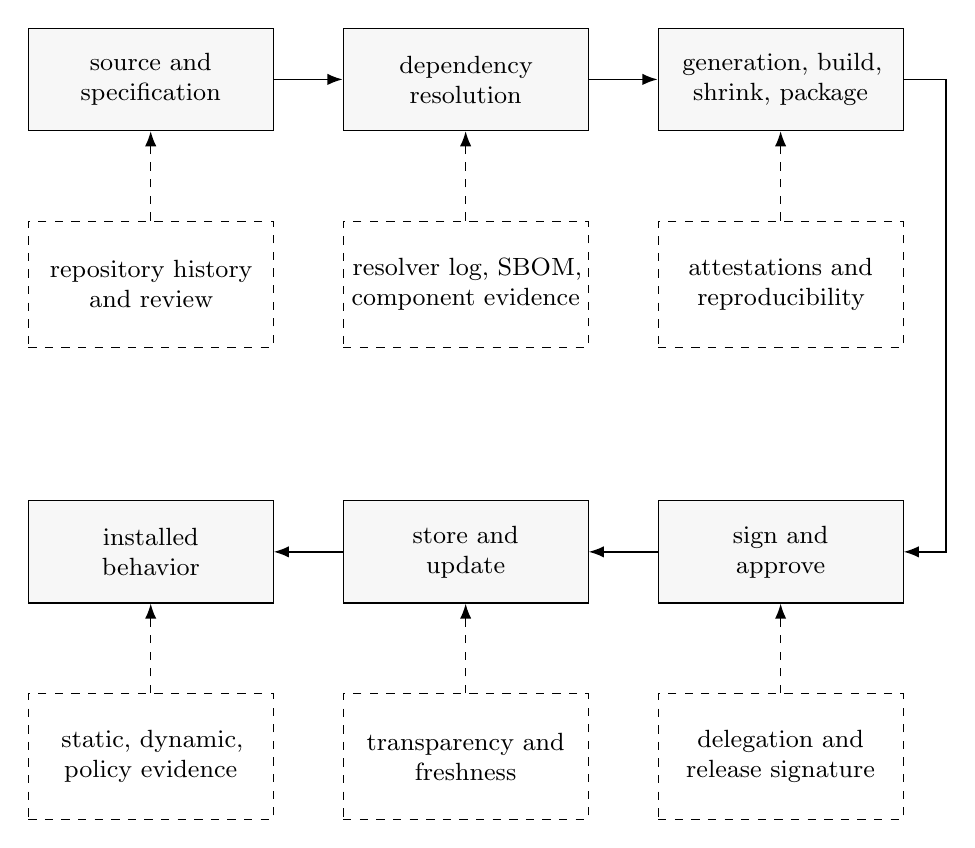
\begin{tikzpicture}[font=\rmfamily\fontsize{9}{10.8}\selectfont,x=1mm,y=1mm,>=Latex,font=\rmfamily\fontsize{9}{10.8}\selectfont\rmfamily,
 stage/.style={draw,align=center,text width=29mm,minimum height=13mm,inner sep=3pt,fill=black!3},
 ev/.style={draw,dashed,align=center,text width=29mm,minimum height=16mm,inner sep=3pt},
 arr/.style={->,line width=.55pt}]
\node[stage] (src) at (0,0) {source and\\specification};
\node[stage] (dep) at (40,0) {dependency\\resolution};
\node[stage] (build) at (80,0) {generation, build,\\shrink, package};
\node[ev] (git) at (0,-26) {repository history\\and review};
\node[ev] (lock) at (40,-26) {resolver log, SBOM,\\component evidence};
\node[ev] (att) at (80,-26) {attestations and\\reproducibility};
\node[stage] (sign) at (80,-60) {sign and\\approve};
\node[stage] (store) at (40,-60) {store and\\update};
\node[stage] (run) at (0,-60) {installed\\behavior};
\node[ev] (auth) at (80,-86) {delegation and\\release signature};
\node[ev] (trans) at (40,-86) {transparency and\\freshness};
\node[ev] (beh) at (0,-86) {static, dynamic,\\policy evidence};
\draw[arr] (src.east)--(dep.west);
\draw[arr] (dep.east)--(build.west);
\draw[arr] (build.east)--(101,0)|-(sign.east);
\draw[arr] (sign.west)--(store.east);
\draw[arr] (store.west)--(run.east);
\draw[arr,dashed] (git.north)--(src.south);
\draw[arr,dashed] (lock.north)--(dep.south);
\draw[arr,dashed] (att.north)--(build.south);
\draw[arr,dashed] (auth.north)--(sign.south);
\draw[arr,dashed] (trans.north)--(store.south);
\draw[arr,dashed] (beh.north)--(run.south);
\end{tikzpicture}
\caption{Cross-layer evidence along an Android lifecycle. Every transition requires an object binding; evidence attached to one stage does not automatically validate another stage.}
\Description{Six lifecycle stages follow two rows: source, dependency resolution, and build run left to right above; signing, store, and installed behavior continue right to left below. Each stage has a corresponding evidence source beneath it: repository history, resolver records, attestations, release authorization, transparency, or behavior analysis.}
\label{fig:lifecycle}
\end{figure}

A minimally useful chain records a source revision, resolved dependency set, build and generation configuration, output APK digest, signing identity, release authorization, and publication event. Artifact analysis can then verify the packaged components and compare the output with prior or disputed artifacts. Behavior analysis evaluates the exact digest. This structure does not guarantee security, but it makes disagreements localizable and claims reviewable.

\section{AI-Mediated Transformations and Mobile Lineage}
\label{sec:ai}

AI-assisted development is not one transformation. It ranges from completion of a few lines to generation of an application skeleton, selection of dependencies, modification across multiple files, test execution, debugging, and release preparation. The relevant provenance question is therefore not merely whether ``AI was used.'' It is which artifact-changing decisions were delegated, which context influenced them, and how the resulting outputs were bound to the final application.

\subsection{From text descriptions to mobile artifacts}

Text2App translates natural-language descriptions through an intermediate representation into Android application code~\cite{text2app}. This pipeline is useful for lineage analysis because it makes several transformations explicit: description to structured representation, representation to source, source to build inputs, and build inputs to APK. A generated application can share layout and behavior with other outputs while containing different source text. Conversely, two descriptions can produce similar source through templates or libraries.

AppForge is an Android development benchmark that evaluates generated projects and coding agents, including compilation-feedback refinement~\cite{appforge}. It supplies a functional evaluation setting, not an authenticated lineage system. In a tool-using workflow, prompts, retrieved material, tool responses, repository state, and accepted revisions can all affect the final output. A final source diff does not record that complete path.

These systems do not make traditional repackaging evidence obsolete. A generated app can itself be copied, repackaged, or combined with existing code. What changes is the space of legitimate relatedness. Multiple authorized outputs may descend from the same prompt, template, or model-mediated plan without one being copied from another. Direction cannot be inferred from pairwise similarity alone.

\subsection{Nondeterminism and reproducibility}

Conventional build reproducibility assumes that a declared input set and deterministic procedure should yield the same bytes. Generative systems may sample different outputs for the same prompt, call external tools, or depend on changing model and retrieval services. Exact reproduction can therefore be unavailable even when the process is authorized.

This does not eliminate reproducibility as an objective; it changes what must be reproduced. One target is \emph{record reproducibility}: an independent verifier can confirm the prompt or specification reference, model or service identity, parameters, tool sequence, retrieved materials, and accepted outputs. Another is \emph{decision replay}: a recorded output is retained and subsequent deterministic build steps reproduce the APK. A third is \emph{distributional replication}: repeated generations satisfy a defined property, which is an empirical model claim rather than artifact lineage.

For mobile supply-chain assurance, preserving the accepted generated source or patch is usually more important than reproducing the model's sampling event. The build attestation should treat that accepted output as a material with a digest. If policy requires regeneration, the record must acknowledge that regenerated code may be a sibling rather than an identical ancestor.

\subsection{Security of generated code}

Studies of code assistants show that generated suggestions can contain security weaknesses and that user interaction affects the result. Pearce et al. evaluated Copilot contributions across security-relevant scenarios~\cite{pearce}. Perry et al. found less secure code in their assisted group, whereas Sandoval et al. found a small security impact in a constrained C task~\cite{perry,sandoval}. Khoury et al. examined ChatGPT-generated code and improvement prompts~\cite{khoury}. The differing tasks, models, participants, and vulnerability oracles preclude a pooled claim that assistance invariably increases insecurity.

For lineage, the important finding is structural: generation provenance does not imply secure behavior. An authorized model-assisted change may introduce a vulnerability; an unauthorized derivative may remove one. Security review must analyze the actual accepted code and built artifact. The provenance record helps identify which model-mediated step introduced a change, but the vulnerability evidence comes from static analysis, testing, review, or formal reasoning.

Human approval also needs careful interpretation. Clicking ``accept'' establishes an interaction event, not necessarily informed review. A policy may require that a maintainer approve generated changes, but the evidential value depends on what was shown, which tests ran, whether warnings were visible, and whether the reviewer had authority for the affected component. Authorization and assurance remain separate.

\subsection{Dependencies and package hallucination}

Generative systems can recommend dependencies by name. Spracklen et al. show that code-generating models can produce nonexistent package names, creating a package-confusion risk when an attacker registers a hallucinated name~\cite{spracklen}. In an Android project, analogous risks can involve Maven coordinates, Gradle plugins, native packages, JavaScript dependencies in hybrid apps, or download URLs. The suggestion may enter source or build configuration even when no copied code appears in the model output.

This risk links AI assistance directly to supply-chain provenance. A robust record should capture the dependency request, resolver result, repository origin, version, integrity digest, and whether the dependency was already approved. A policy can reject unrecognized repositories or require lockfile review. Binary component analysis then checks whether the resolved material appears in the APK. Neither the prompt log nor the binary detector alone provides the full chain.

Package hallucination also creates a novel counter-history for library attribution. A newly registered malicious package may intentionally implement an interface or name suggested by a model. The package's code is not necessarily similar to an established library, so clone detection may not flag it. Repository provenance, registration chronology, maintainer identity, and dependency-policy evidence become central.

\subsection{Training-data and privacy lineage}

CodexLeaks demonstrates that code-generation models can emit sensitive information associated with training data~\cite{codexleaks}. The resulting lineage question differs from ordinary source copying. A generated fragment may be statistically or verbatim related to training material whose exact membership is unavailable. A final application can therefore contain sensitive or proprietary material without a normal repository-level copy event.

Artifact similarity can still help when a suspected source is known, but absence of a match is weak evidence because generation may transform names and structure. Provenance records can establish which model and prompt produced the accepted output, yet they may not reveal the relevant training example. Policy and legal conclusions require evidence beyond technical resemblance, including license, confidentiality, and permitted-use analysis.

Privacy also affects what provenance should retain. Storing complete prompts, retrieved files, and model outputs may itself expose secrets. A mobile-development provenance design should support selective disclosure: retain cryptographic commitments, access-controlled detailed records, and public metadata sufficient to bind the final artifact without publishing sensitive context. The record needs an evidence-retention policy, not indiscriminate logging.

\subsection{Multi-principal and tool-mediated authorship}

An agentic workflow can include a human requester, model provider, model instance, retrieval source, code repository, build service, package registry, test system, reviewer, and release signer. These are not equivalent principals. The model service may produce candidate text but lack release authority. A human may approve a patch but not control the signing key. A build service may emit an attestation but not own the source.

Supply-chain layouts are well suited to representing these roles when model-mediated steps are treated as explicit transformations. The layout can require that generated outputs pass tests, static checks, dependency policy, and human review before signing. It can also distinguish advisory output from accepted material. This is more precise than adding one boolean ``AI-generated'' field to the APK metadata.

The same role separation helps incident response. If a vulnerability is found, investigators can ask whether it originated in a generated patch, retrieved example, dependency recommendation, manual edit, or build-time transformation. The answer guides remediation and model or policy changes. Without step records, the final Git history may collapse several causes into one commit.

\begin{table}[t]
\caption{AI-mediated development risks and the evidence needed to reason about them.}
\label{tab:ai-risks}
\footnotesize
\begin{tabularx}{\textwidth}{L{2.35cm}Y Y L{1.6cm}}
\toprule
Risk or ambiguity & Why final-artifact similarity is insufficient & Complementary evidence & Main claim \\
\midrule
Sibling generations from one specification~\cite{text2app,appforge} & Similarity does not reveal whether one output copied another & Specification binding, generation records, accepted-output digests & \claimlevel{3}--\claimlevel{4} \\
Insecure generated code~\cite{pearce,perry,sandoval,khoury} & Origin says nothing about security of accepted behavior & Static/dynamic analysis, tests, review evidence, exact artifact binding & \claimlevel{6} \\
Hallucinated dependencies~\cite{spracklen} & Malicious package may be novel and not resemble a known library & Resolver provenance, repository identity, lockfile, component verification & \claimlevel{1}+\claimlevel{4} \\
Training-data or privacy leakage~\cite{codexleaks} & Relevant ancestor may be unknown or transformed & Model/prompt record, similarity investigation, access-controlled context & Conditional \claimlevel{3} \\
Agentic multi-file edits~\cite{appforge} & One final diff hides intermediate tool calls and rejected outputs & Step attestations, tool transcripts, policy checkpoints & \claimlevel{4}--\claimlevel{5} \\
Nondeterministic regeneration & Exact output may not be reproducible from a prompt alone & Preserve accepted output; separate record replay from model replication & \claimlevel{0}+\claimlevel{4} \\
\bottomrule
\end{tabularx}
\end{table}

\subsection{A minimum evidence record for generated transformations}

A generated transformation record should identify: the parent source revision; task or specification identifier; model or service identity at the granularity available; generation parameters; tool and retrieval accesses; candidate-output digests; the accepted patch or file digests; tests and analyses run; human or policy approvals; and the downstream build product. Sensitive context can be access controlled, but the public or shared record should still bind the accepted output to the final APK.

This record serves three purposes. It establishes direction from a parent revision to an accepted generated change. It separates generation from approval and release. It gives artifact and behavior analyses exact objects to examine. The record does not prove that the model never used unrecorded training material or that the accepted code is secure. It makes those residual questions explicit rather than hiding them behind a generic provenance claim.

\section{Cross-Layer Synthesis: What the Evidence Can Establish}
\label{sec:synthesis}

The preceding literatures solve different parts of one problem. Android comparison methods observe the final artifact and recover relations that process records may omit. Component analysis separates first-party logic from dependencies and identifies versions. Supply-chain mechanisms record and authorize production steps. Behavioral analyses evaluate security and policy properties. AI-mediated workflows add transformations whose context may not be represented in source history. The synthesis question is how these observations combine without allowing one layer to stand in for another.

\subsection{Six invalid substitutions}

Six recurring substitutions expose the missing premise between available evidence and the operationally desired claim:

\begin{enumerate}
\item \textbf{Similarity for direction.} A match cannot by itself distinguish $A\rightarrow B$, $B\rightarrow A$, or a common predecessor; chronology, source, ownership, a deployed mark, or an attested transformation must supply the asymmetry.
\item \textbf{Signer for authorized publisher.} A signature binds an artifact to a key. Authorization additionally binds that key to a scoped role, validity interval, and policy; delegation and transparency systems provide such context~\cite{tuf,diplomat,sigstore}.
\item \textbf{Provenance for benign behavior.} An attestation can bind declared inputs and a build to a digest while faithfully recording a vulnerable or malicious result. The exact artifact still requires behavior-specific analysis.
\item \textbf{Component presence for exploitability.} A family, version, or SBOM match does not establish that affected code is present, reachable, configured, and exposed; non-detection also does not prove absence after shading, shrinking, patching, or dynamic loading.
\item \textbf{Reproducibility for approval.} Independent builders can reproduce an unauthorized output from unauthorized declared inputs. Reproducibility strengthens equality and source-to-binary binding, not input policy.
\item \textbf{Generation log for complete causal history.} Prompts and responses may omit retrieval, tool state, rejected candidates, manual edits, or downstream transforms. The record must bind the accepted output, parent, and final artifact at the granularity required by the claim.
\end{enumerate}

These are evaluation errors, not merely wording errors. An oracle can already encode direction, an honest-functionary prototype can hide compromised behavior, and full upstream packages can make versioning appear easier than partially packaged code. Reporting the missing premise identifies the hard negatives a study must include.

\subsection{A cross-layer assurance pattern}

Figure~\ref{fig:assurance-case} presents a reusable assurance pattern. It is not a mandatory architecture. It is a claim graph that identifies the minimum bindings needed when an analyst wants to assert that a released Android artifact is an authorized product of a declared process and satisfies a stated property.

\begin{figure}[t]
\centering
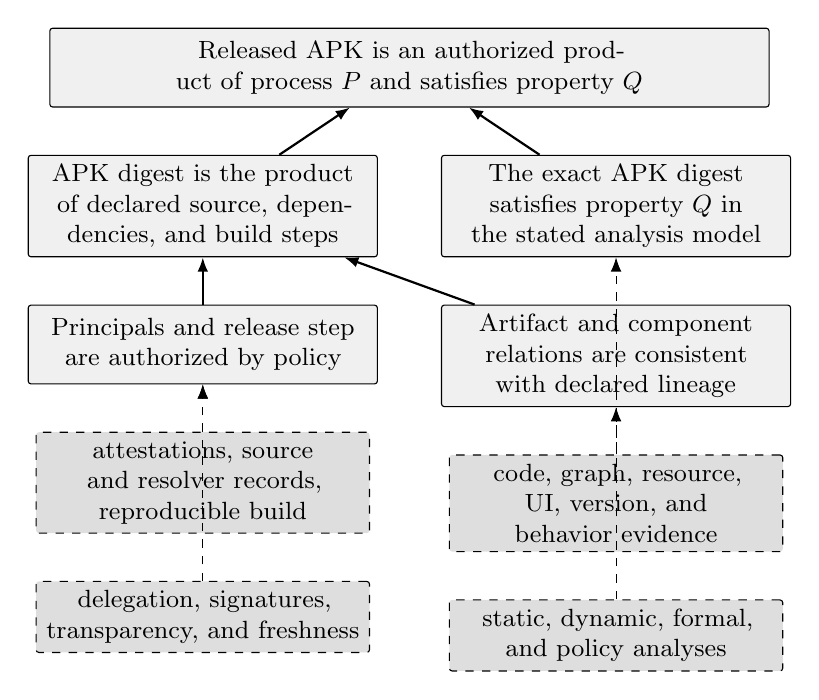
\begin{tikzpicture}[
  c/.style={draw,rounded corners=1pt,align=center,text width=4.2cm,minimum height=10mm,fill=black!6,font=\small},
  e/.style={draw,dashed,rounded corners=1pt,align=center,text width=4.0cm,minimum height=9mm,fill=black!13,font=\small},
  arr/.style={-{Latex[length=1.8mm]},thick},
  sup/.style={-{Latex[length=1.8mm]},dashed},
  node distance=6mm and 8mm
]
\node[c,text width=8.9cm] (top) {Released APK is an authorized product of process $P$ and satisfies property $Q$};
\node[c,below left=6mm and 4mm of top.south] (prov) {APK digest is the product of declared source, dependencies, and build steps};
\node[c,below right=6mm and 4mm of top.south] (beh) {The exact APK digest satisfies property $Q$ in the stated analysis model};
\node[c,below=of prov] (auth) {Principals and release step are authorized by policy};
\node[c,below=of beh] (rel) {Artifact and component relations are consistent with declared lineage};
\node[e,below=of auth] (att) {attestations, source and resolver records, reproducible build};
\node[e,below=of rel] (sim) {code, graph, resource, UI, version, and behavior evidence};
\node[e,below=of att] (sig) {delegation, signatures, transparency, and freshness};
\node[e,below=of sim] (ana) {static, dynamic, formal, and policy analyses};
\draw[arr] (prov)--(top);\draw[arr] (beh)--(top);\draw[arr] (auth)--(prov);\draw[arr] (rel)--(prov);
\draw[sup] (att)--(auth);\draw[sup] (sig)--(auth);\draw[sup] (sim)--(rel);\draw[sup] (ana)--(beh);
\end{tikzpicture}
\caption{Cross-layer assurance pattern. Solid arrows are subclaims; dashed arrows are evidence. Every evidence item must bind to the same artifact digest or to a documented predecessor relation.}
\Description{A top claim that an APK is authorized and satisfies a property is supported by provenance and behavior branches. Lower boxes show authorization, declared lineage, attestations, signatures, similarity evidence, and program analyses.}
\label{fig:assurance-case}
\end{figure}

The top claim has two independent branches. The provenance branch asks whether the APK is the product of the declared process and whether that process was authorized. The behavior branch asks whether the exact APK satisfies property $Q$. Artifact and component analyses cross-check the declared lineage rather than merely repeating it. A mismatch does not automatically select which source is wrong; it triggers investigation.

This pattern accommodates incomplete provenance. If no trustworthy process record exists, artifact comparison may provide the best available evidence of relationship, but the top claim must be weakened. If the build is fully attested but behavior analysis is absent, the lineage claim can be strong while the security claim remains open. Reporting partial assurance is more informative than forcing a binary verdict.

\subsection{Binding rules}

Cross-layer evidence is useful only when records refer to the same objects. Four binding rules are therefore central.

\begin{enumerate}
\item \textbf{Digest binding.} Every attestation, signature, store record, component report, and behavior result should name the artifact digest it covers. Package names and version strings are insufficient because they can be reused or equivocated.
\item \textbf{Predecessor binding.} When artifacts are intentionally non-identical, the record should name the transformation and parent digest. A similarity score alone should not be used as the link when a process record can supply one.
\item \textbf{Principal binding.} Keys, accounts, model services, builders, and reviewers should be mapped to scoped roles and validity intervals. ``Signed'' is not a complete identity statement.
\item \textbf{Policy binding.} Authorization and behavior conclusions should name the policy version or property definition. A decision can change when the policy changes even if the artifact does not.
\end{enumerate}

These rules also improve reproducibility. A later reviewer can determine whether two analyses disagree because they used different APKs, different component databases, different policies, or different environments. Without the bindings, disagreement is difficult to localize.

\subsection{Contradiction patterns}

A synthesis should preserve contradictions rather than averaging them away. Five patterns are particularly important.

\paragraph{Incompatible denominators.}
One study may report the fraction of known positive pairs detected, another the fraction of returned pairs judged positive, and a third classification accuracy on balanced data. The numbers cannot be ranked without reconstructing the denominators. This issue is prominent in repackaging evaluations and motivates the RePack effort~\cite{repack}.

\paragraph{Different transformation distributions.}
A method may appear robust because its benchmark contains renaming and packing but not control-flow restructuring or resource replacement. Another may target a different set. The correct synthesis is a coverage matrix, not a single robustness ordering.

\paragraph{Different objects.}
A library detector can report classes, modules, families, or versions. A clone detector can report methods, applications, pairs, or clusters. A supply-chain system can report steps, targets, or releases. Claims using different objects should not be counted as direct replications.

\paragraph{Different oracle provenance.}
Controlled transformations provide precise lineage labels but limited realism. Market-derived labels provide realism but uncertain ground truth. Authenticated process records provide direct history for participating projects but may not exist for adversarial artifacts. Each oracle closes one gap and opens another.

\paragraph{Different threat models.}
A signature scheme can be correct when keys are uncompromised; a delegation system may tolerate some compromised roles; a transparency system targets equivocation; a detector targets transformed copies; and a behavior analysis targets malicious functionality. Calling all of them ``supply-chain security'' does not make their guarantees interchangeable.

Table~\ref{tab:contradictions} turns these patterns into reporting obligations.

\begin{table}[t]
\caption{Contradiction patterns and the information needed to resolve or bound them.}
\label{tab:contradictions}
\small
\begin{tabularx}{\textwidth}{L{2.7cm}Y Y}
\toprule
Observed disagreement & Likely hidden difference & Required report \\
\midrule
Different accuracy or recall & Candidate universe, class balance, threshold, pair construction & Counts by unit, full confusion matrix or retrieval curve, threshold-selection procedure \\
Different obfuscation robustness & Transformation operators, strength, order, and composition & Transformation matrix and per-operator results \\
Different library-version results & Database coverage, module granularity, shrinkage, forks & Candidate versions, unknown state, observed/missing discriminators \\
Attestation and binary scan disagree & Undeclared dependency, detector miss, post-build change, wrong digest & Exact materials, product digest, detector database, packaging step \\
Signature valid but release disputed & Key compromise, expired role, wrong scope, account takeover & Delegation chain, validity interval, transparency and revocation state \\
Generated output cannot be reproduced & Nondeterminism, model drift, retrieval change, missing tool state & Accepted-output digest, model/service record, tool transcript, replay boundary \\
\bottomrule
\end{tabularx}
\end{table}

\subsection{An evaluation blueprint}

A cross-layer evaluation should be organized around falsification. It must name the object and proposition; retain positive, hard-negative, and unknown cases; separate candidate retrieval from verification; include ordered transformation compositions; split by family, developer, market, and time; and recheck a sample of all label states. For generated artifacts, outputs from one prompt family, seed project, or trajectory belong in one partition. For component and vulnerability claims, presence, exact version, reachability, and observed exploit conditions remain separate.

Operational reporting must include candidate volume, abstention, explanation size, and adjudication effort. Every downstream component, behavior, provenance, or authorization result must bind to the same APK digest or a documented predecessor relation. Table~\ref{tab:checklist} turns these requirements into a minimum report; it is a floor rather than a complete domain-specific protocol.

\begin{table}[t]
\caption{Minimum reporting checklist for evidence-centered Android lineage evaluation.}
\label{tab:checklist}
\small
\begin{tabularx}{\textwidth}{L{2.7cm}Y Y}
\toprule
Area & Required information & Failure prevented \\
\midrule
Claim & Object, relation, claim level, assumptions & Similarity or signature promoted to a stronger claim \\
Corpus & Source, dates, markets, counts by unit, inclusion and unknowns & Hidden base rates and irreproducible denominators \\
Oracle & Label construction, direction source, recheck procedure & Circular evaluation and false certainty \\
Transformations & Operators, parameters, composition, ordinary vs adversarial & Vague robustness claims \\
Components & Library handling, version database, partial/unknown state & Common-code false positives and overconfident versioning \\
Provenance & Materials, steps, principals, product digests, layout or policy & Records that cannot be linked to the analyzed APK \\
Authorization & Role scope, validity, delegation, revocation, transparency & Treating any valid key as rightful publisher \\
Behavior & Property, tool/model, environment, coverage, limitations & Treating provenance as security assurance \\
AI mediation & Accepted-output digest, model/service, context boundary, tools, review & Unreplayable or misleading generation history \\
Operations & Candidate volume, latency, explanation and human review cost & Laboratory metrics that do not scale to deployment \\
\bottomrule
\end{tabularx}
\end{table}

\subsection{Evidence profiles instead of universal rankings}

The synthesis suggests reporting an evidence profile for each system. A profile is a vector over object granularity, claim level, transformation coverage, oracle strength, corpus transfer, and explanation. It avoids a universal ranking that would compare unlike goals. A fast UI detector may be the best first-stage signal for brand impersonation even if it does not establish source derivation. A cryptographic attestation may be decisive for an enrolled build while being irrelevant to an uncooperative third-party clone. A static analyzer may provide the strongest available privacy evidence while saying nothing about authorship.

Evidence profiles also expose combinations. A deployment can select complementary systems whose failure boundaries differ. For example, component-aware code matching can suppress common-library false positives; a release log can provide direction; a delegated signature can provide authorization; and static/dynamic checks can evaluate behavior. The combination should be tested end to end because errors propagate: a wrong component boundary changes the similarity score, a wrong digest breaks provenance binding, and a stale policy changes authorization.

\subsection{What the combined literature supports}

The literature strongly supports four bounded conclusions. First, Android artifact resemblance can be measured through several feature families, but robustness is transformation specific and open-world ground truth is difficult~\cite{repack,droidmoss,andarwin,codematch,viewdroid}. Second, third-party-library evidence is necessary to interpret both similarity and vulnerability claims, yet family, version, and reachability are distinct tasks~\cite{tpl,libscout,atvhunter,keepupdated}. Third, supply-chain mechanisms can preserve direction, principal, authorization, and publication evidence that artifact comparison cannot recover reliably~\cite{tuf,intoto,chainiac,sigstore}. Fourth, AI-mediated development expands the set of transformations and principals while introducing dependency, security, and privacy risks that must be bound to accepted outputs~\cite{text2app,pearce,spracklen,codexleaks}.

The literature does not support a claim that one detector, signature, SBOM, attestation, or AI-disclosure field solves mobile lineage. It supports a layered case in which each observation is limited to the proposition it measures. That limitation is not a weakness of the survey; it is the main design principle for future systems.

\section{Research Agenda and Conclusion}
\label{sec:agenda}

The agenda shifts from a universal repackaging score to reviewable claims about artifact relations, production history, authority, and behavior. Detector evaluations should state the conclusion enabled and the premise supplied elsewhere.

\subsection{Direction-labeled, transformation-complete benchmarks}

Benchmarks should distinguish direct copy, common predecessor, shared library or template, legitimate version, independent generation, and authorized variant. They should record parent/child digests, ordered transformations, first-party/component regions, signing identities, chronology, and label provenance, while separating exact-history controlled cases from realistic field cases and retaining an unknown state.

Android pipelines combine shrinking, desugaring, generation, resource processing, cross-platform compilation, native code, and protection. Because order changes observability, lawful benchmarks should retain per-stage artifacts and report which relation survives each composition.

\subsection{Provenance-to-APK and component-to-behavior binding}

An Android provenance profile should terminate at the analyzed APK, binding source revision, resolved dependencies, generation/build configuration, builder, signer, publication event, and digest. Sensitive details may remain controlled, but commitments and predecessor relations must be checkable.

Declared composition should be reconciled with the binary. Reports must separate family, candidate version, partial inclusion, modification, reachability, and unknowns; reproducible builds, binary comparison, and transparency should act as independent checks rather than repeated declarations.

\subsection{Auditable generated transformations}

AI-mediated development needs artifact-level provenance. Each accepted patch or file set should bind a parent revision to a downstream product and record the model/service boundary, material retrieval/tool context, review decision, output digest, and unavailable evidence. Research must determine how to commit to sensitive context, retain sufficient agent history, cluster sibling generations without asserting copying, verify package recommendations, and represent model or tool drift when replay is impossible.

\subsection{Open-world, temporal, and uncertainty-aware evaluation}

Relatives, developers, libraries, markets, prompt families, and agent trajectories must not leak across random splits. Evaluations should hold out time and entity families, report candidate volume and abstention, keep unknown histories unknown, and distinguish absent, undetected, out-of-scope, and unavailable evidence.

Because keys, roles, packages, policies, and vulnerabilities change, decisions should be reproducible at a stated time and revisable through append-only records and explicit policy versions.

\subsection{Decision-centered assurance tooling}

Tooling should ingest artifact, component, provenance, signature, transparency, policy, and behavior evidence; check digest/predecessor bindings; and report supported, contradicted, and unresolved subclaims rather than one trust score.

Evaluation should follow retrieval, localization, adjudication, policy action, and appeal. With candidate population, policy, time, and review budget fixed, comparisons should test artifact-only, process-only, and bound cross-layer evidence and report precision/recall, abstention, reviewer effort, binding success, and localized disagreements. A decision log should also preserve the evidence available at the time, the policy version, the reason for abstention or escalation, and any later evidence that changed the outcome. Such revision tests whether the system supports accountable correction rather than only one-shot classification.

\subsection{Stewardship and practice}

AndroZoo and RePack show the value of shared data~\cite{androzoo,repack}. Resources should preserve label provenance, transformations, licenses, errors, and historical denominators; constrained evaluations can separate public synthetic, redistributable open-source, metadata-only field, and controlled-access strata.

Stores should separate retrieval, lineage, authorization, and behavior review. Developers should retain source-to-APK/dependency bindings, protect signing roles, preserve analyzed artifacts, and record accepted generated changes. Researchers should report the claim ceiling rather than overstate direction or authority.

\subsection{Conclusion}

Android lineage comprises identity, composition, resemblance, derivation, process, authority, and behavior. Repackaging, TPL, supply-chain, and AI-development research illuminate different links; none should be promoted beyond its observation.

A defensible assurance case binds source and dependencies to build steps, steps to an APK digest, the digest to an authorized transparent release, and the exact artifact to component and behavior analyses. Artifact comparison remains essential when records are absent or disputed; provenance supplies direction and accountability. This claim-centered structure is a stronger target than a universal repackaging score.


\bibliographystyle{ACM-Reference-Format}
\bibliography{references}
\end{document}
